\begin{figure}[htbp]
\section*{ CNTNAP2}
\centering
\begin{subfigure}[b]{0.95\textwidth}
\centering
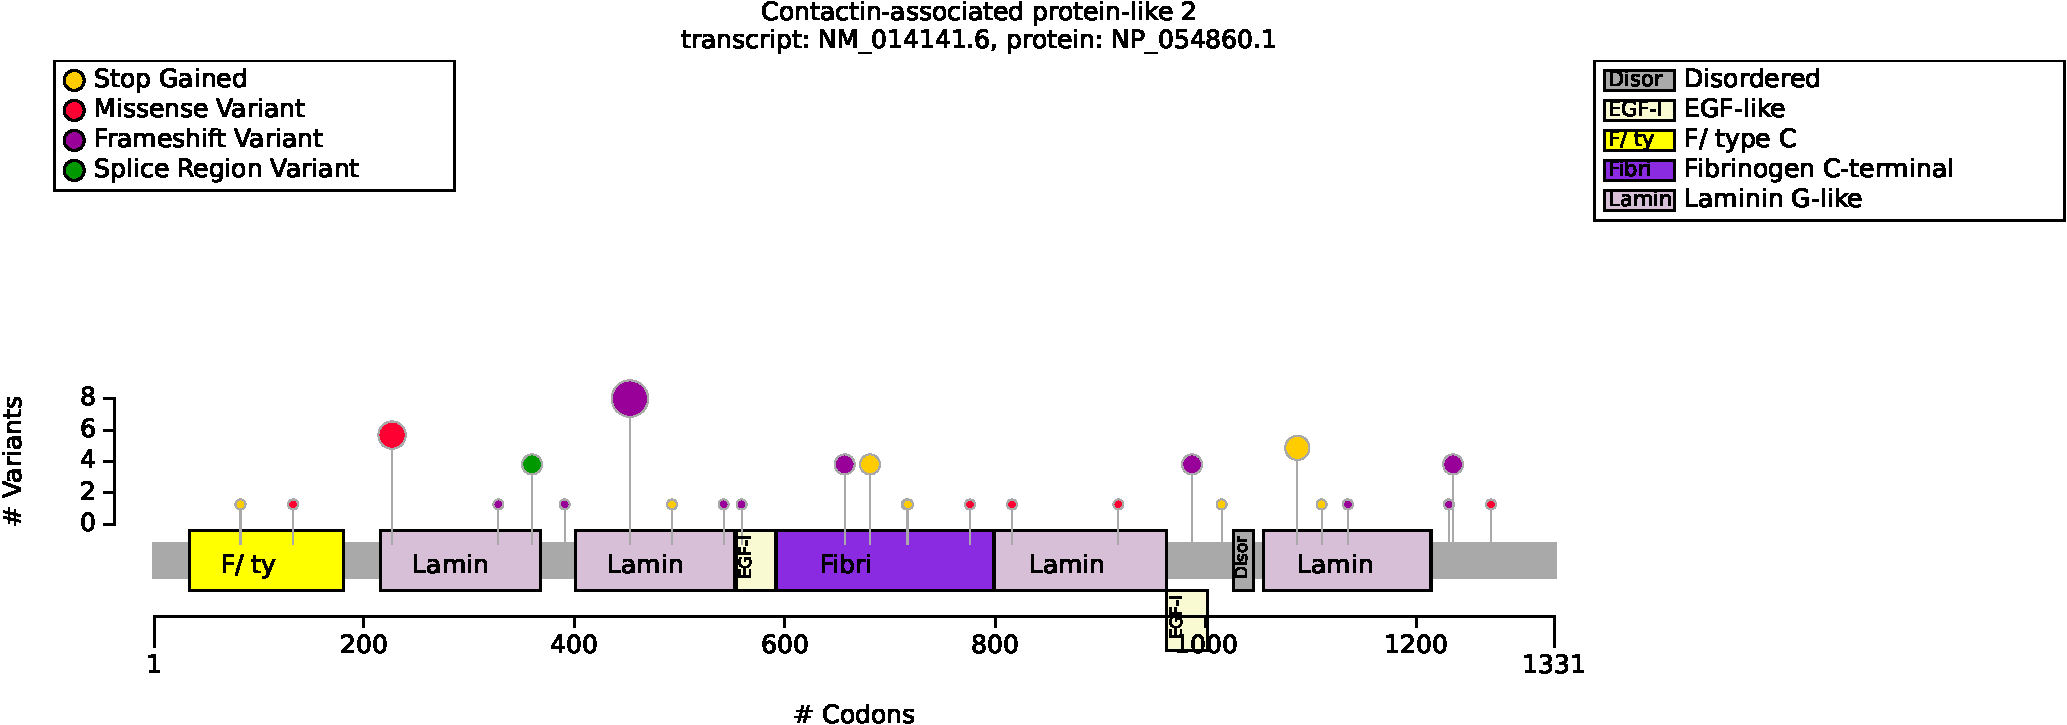
\includegraphics[width=\textwidth]{ img/CNTNAP2_protein_diagram.pdf} 
\captionsetup{justification=raggedright,singlelinecheck=false}
\caption{Distribution of variants in CNTNAP2}
\end{subfigure}

\vspace{2em}

\begin{subfigure}[b]{0.95\textwidth}
\centering
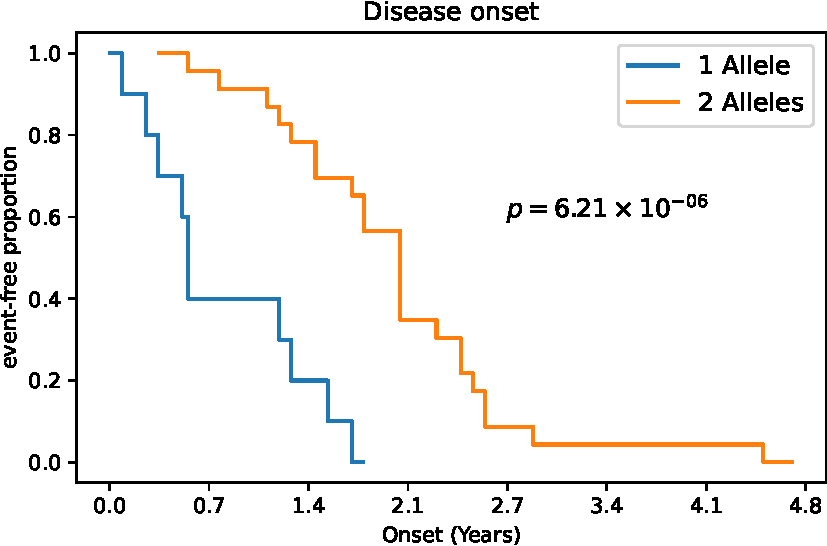
\includegraphics[width=0.3\textwidth]{ img/CNTNAP2_stats.pdf} 
\captionsetup{justification=raggedright,singlelinecheck=false}
\caption{TODO adapt caption CNTNAP2}
\end{subfigure}

\vspace{2em}

\begin{subfigure}[b]{0.95\textwidth}
\centering
\resizebox{\textwidth}{!}{
\begin{tabular}{llllrr}
\toprule
Genotype (A) & Genotype (B) & total tests performed & significant results\\
\midrule
Ablation/Ablation & other/other OR Ablation/other & 16 & 0\\
FEMALE & MALE & 15 & 0\\
1 & 2 & 11 & 0\\
\bottomrule
\end{tabular}
}
\captionsetup{justification=raggedright,singlelinecheck=false}
\caption{Fisher Exact Test performed to compare HPO annotation frequency with respect to genotypes.}
\end{subfigure}

\vspace{2em}

\begin{subfigure}[b]{0.95\textwidth}
\captionsetup{justification=raggedright,singlelinecheck=false}
\resizebox{\textwidth}{!}{
\begin{tabular}{llllrr}
\toprule
Description & Variable & Genotype (A) & Genotype (B) & p-value & xrefs\\
\midrule
Compute time until OMIM:610042 onset & Onset of OMIM:610042 & 1 & 2 & $6.21\times 10^{-6}$ & -\\
\bottomrule
\end{tabular}
}
\caption{Onset of OMIM:610042 to compare 1 and 2 with respect to Onset of OMIM:610042.}
\end{subfigure}

\vspace{2em}

\caption{The cohort comprised 63 individuals (29 females, 32 males, 2 with unknown sex). 
2 of these individuals were reported to be deceased. A total of 72 HPO terms were used to 
annotate the cohort. Disease diagnosis: Pitt-Hopkins like syndrome 1 (OMIM:610042). 
D'Onofrio et al. (2023) reported several GPCs, but the authors did not
apply multiple-testing correction \cite{PMID_37183190}. These authors did not perform survival analysis for age of onset of disease.
A total of 74 unique variant alleles were found in \textit{CNTNAP2} (transcript: \texttt{NM\_014141.6}, protein id: \texttt{NP\_054860.1}).}
\end{figure}
